\chapter{Apache Spark Internals}

\section{Introduction and Motivations}
	\par
	From a \textbf{software engineering} point of view the Hadoop \textbf{code base} is huge (while Spark's is smaller) and contributions/extensions are cumbersome.
	\newline
	\par\noindent
	From a \textbf{system/framework} point of view Spark is better because of its \textbf{unified pipeline}:
	\begin{itemize}
		\item Spark Streaming for stream processing
		\item GraphX for graph processing
		\item MLLib, Machine Learning Library
		\item Spark SQL for SQL on Spark
	\end{itemize}
	And its simplified data flow and faster processing speed (Spark is faster not only because of the simplified data flow, but also because it \textbf{avoid materializing data on HDFS} after each iteration).
	\newline
	\par\noindent
	From a \textbf{data abstraction} point of view Spark introduces a new fundamental abstraction: the \textbf{RDDs}. They are easy to extend with new operators and there is a more descriptive computing model. Computation is organized in multiple stages: \textbf{Transformations} apply user code to distributed data in parallel while \textbf{Actions} assemble final output of an algorithm, from distributed data.
\section{Anatomy of a Spark Application}
	\par
	\begin{figure}[H]
		\centering
		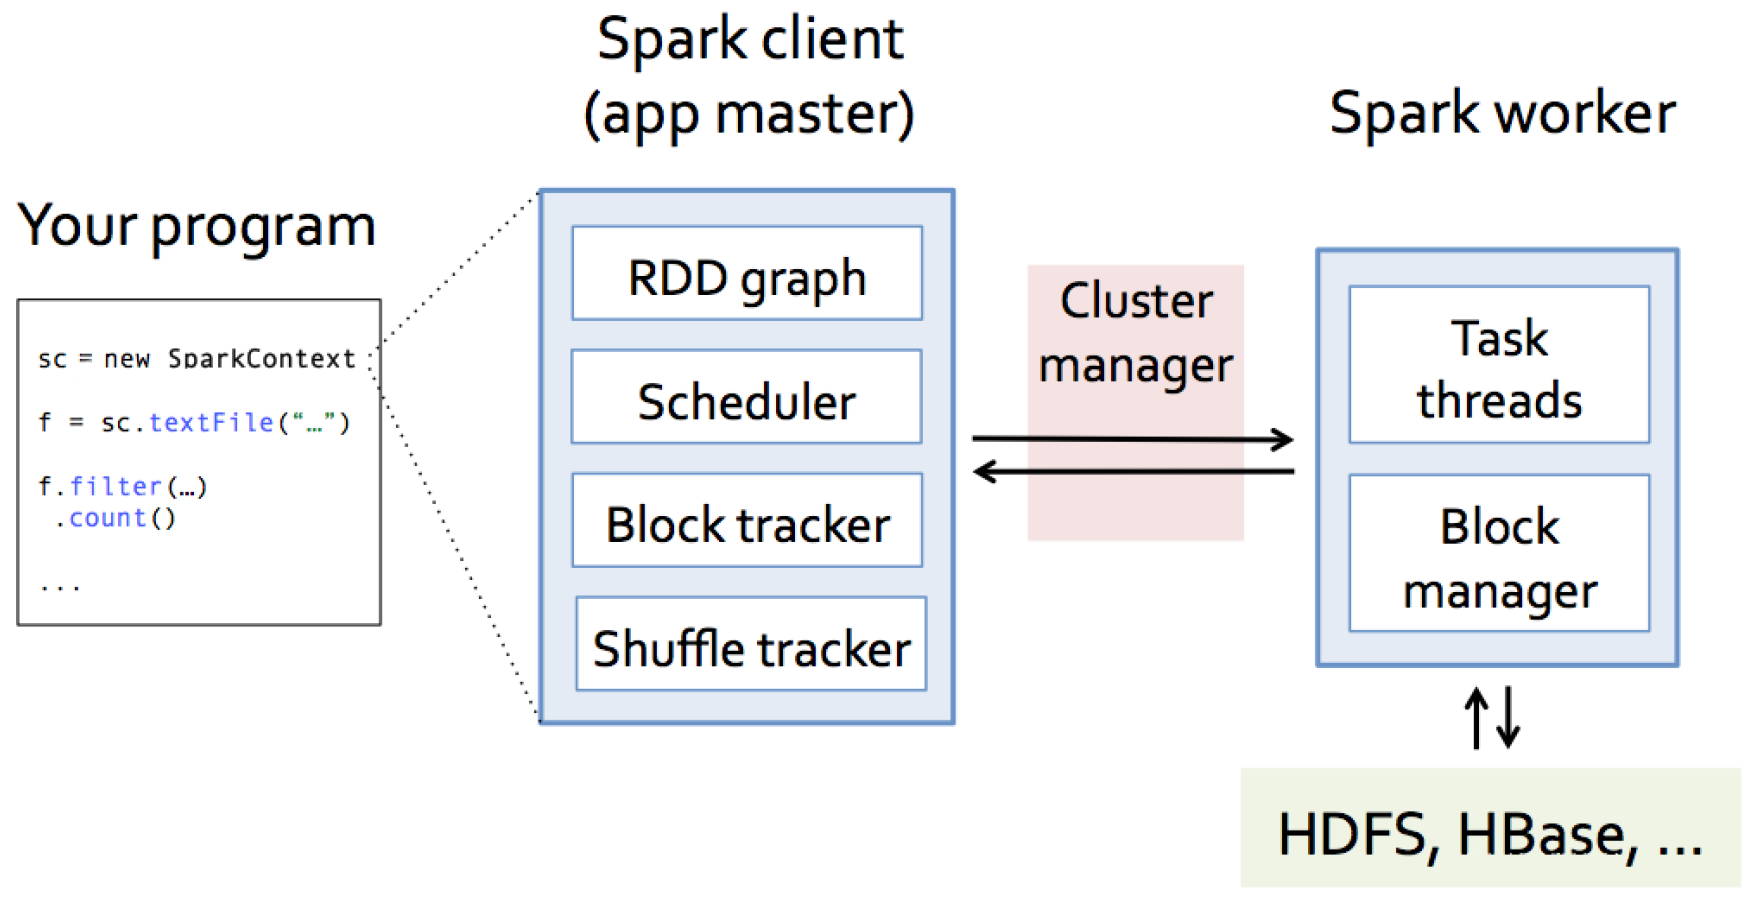
\includegraphics[width=\linewidth]{images/sparkcomp.png}
		\caption{\textit{Spark components details.}}
	\end{figure}
	Spark applications respect the same locality principle as Hadoop and use caching for filtered RDDs.
	\newline
	A generic application creates a \textbf{SparkContext} which is a core component of the \textbf{DriverProgram}, then it registers to the \textbf{ClusterManager}. Upon an action, the driver program submits the job to the cluster manager.
	\newline
	The \textbf{Cluster Manager} does not know about stages, it starts executors on workers nodes.
	\newline
	The \textbf{RDD objects} build the operator for the Directed Acyclic Graph (\textbf{DAG}).
	\newline
	The \textbf{DAG Scheduler} splits the DAG into stages of tasks (	lazy evaluation model) and submits each stage and its task as they are ready to the task scheduler, it uses a listener for the results.
	\newline
	The \textbf{Task Scheduler} launch tasks on \textit{executors} via Master and retries failed and straggler tasks, it reports to the DAG scheduler.
	\newline
	The \textbf{Worker} launches spark executor in a process, tasks are launched in separate threads, one per each core on the worker node.
	\begin{figure}[H]
		\centering
		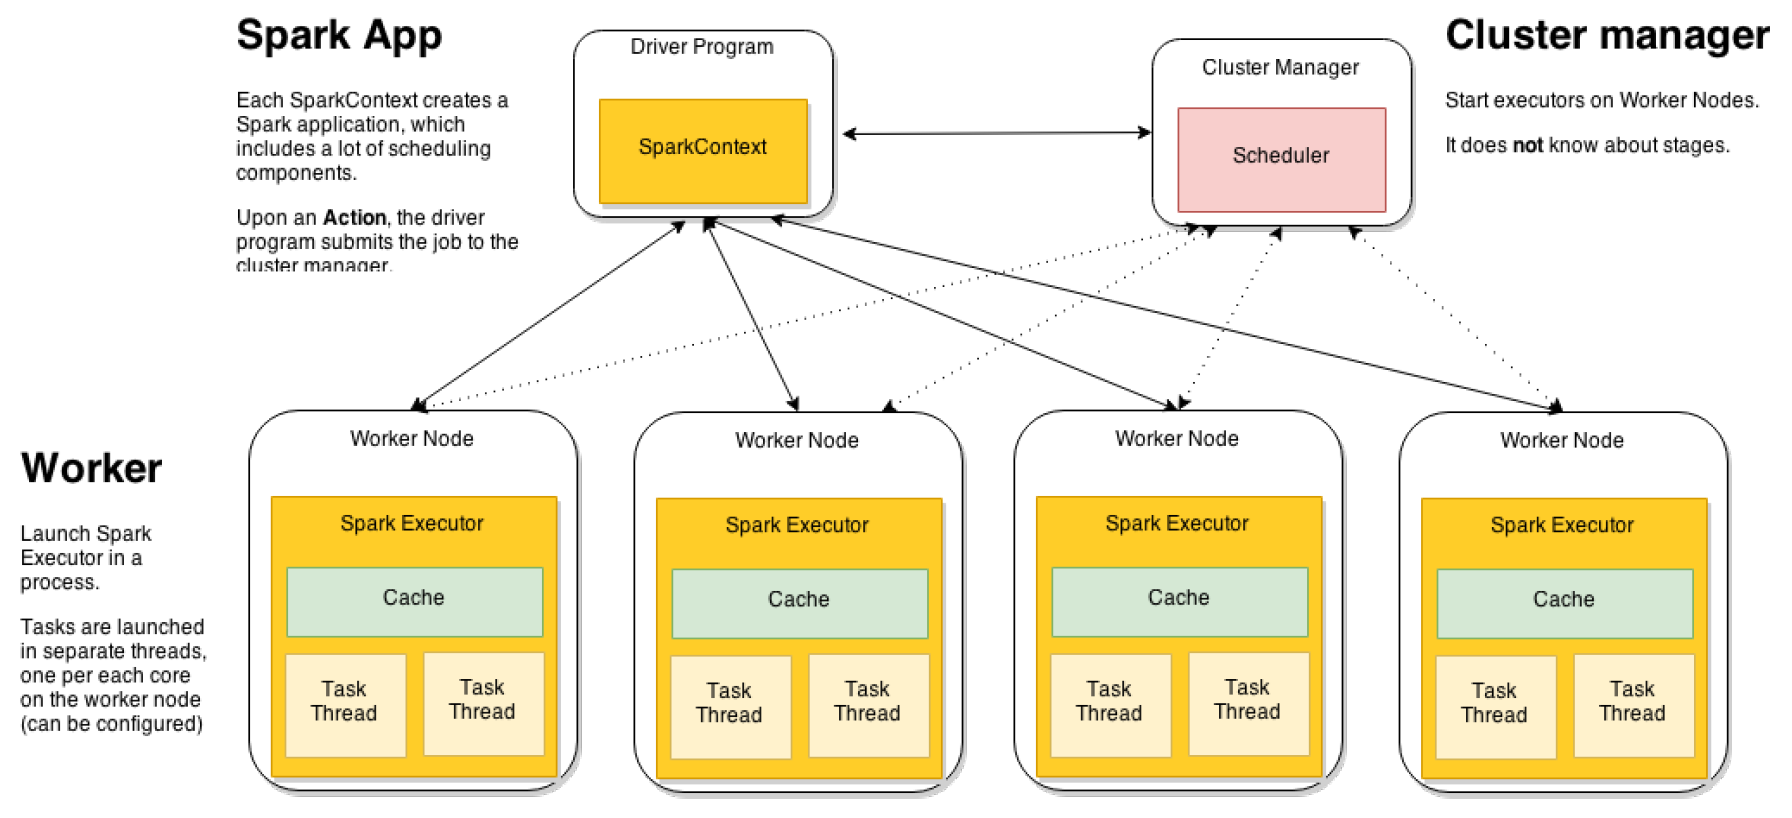
\includegraphics[width=\linewidth]{images/sparkcompsys.png}
		\caption{\textit{Spark components: system level view.}}
	\end{figure}
\section{Spark Deployments}
	\par
	The general workflow of a Spark application is the following:
	\begin{enumerate}
		\item The Spark application creates a \textbf{SparkContext}, which initializes the \textbf{DriverProgram}
		\item It registers to the \textbf{ClusterManager}
		\item It asks resources to allocate executors
		\item It schedules Task execution
	\end{enumerate}
	The master node is the machine running the Master program and the Driver (SparkContext and application code).
	\newline
	The worker nodes are machines that run executors. They host one or multiple Workers with one JVM (1 UNIX process) per each one. Each Worker can spawn one or more Executors.
	\newline
	The Executors run tasks. They run in child JVM (1 UNIX process) and execute the tasks using threads in a \textit{ThreadPool}
	\begin{figure}[H]
		\centering
		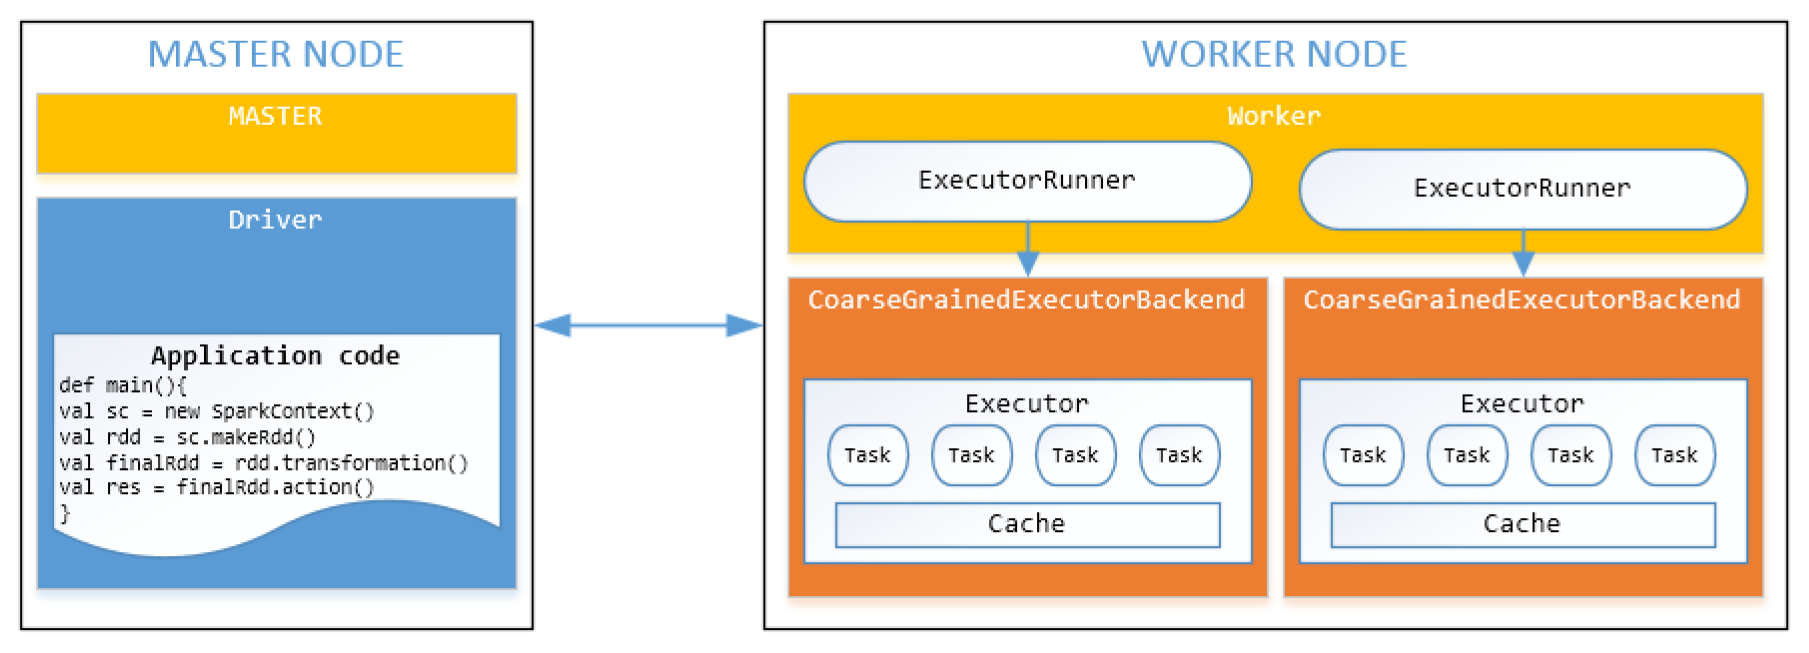
\includegraphics[width=\linewidth]{images/masterworker.png}
		\caption{\textit{Master node and Worker nodes.}}
	\end{figure}
	\begin{table}[H]
		\centering
		\begin{tabular}{p{0.47\linewidth}p{0.47\linewidth}}
			\textbf{Hadoop} & \textbf{Spark} \\ \hline
			One task per UNIX process (JVM), more if there is JVM reuse. & Tasks run in one or more threads within a single UNIX process (JVM). \\ \hline
			Use MultiThreadedMapper advanced feature to have threads in Map tasks. & Executor process is statically allocated to worker, even with no threads. \\ \hline
			\textbf{Short-life executor with one large task.} & \textbf{Long-life executor with many small tasks.} \\ \hline
		\end{tabular}
	\end{table}
	\subsection{Benefits of the Spark architecture}
		\subsubsection{Isolation}
			\par
			Applications are completely isolated, task scheduling per application.
		\subsubsection{Low-overhead}
			\par
			The task setup cost is that of spawning a thread, not a process. Small tasks mitigate the effects of data skew (difference in the distribution of data).
		\subsubsection{Sharing data}
			\par
			Applications cannot share data in memory natively, they use an external storage service like a distributed caching mechanism to store and share RDDs in memory.
		\subsubsection{Resource allocation}
			\par
			Static process provisioning for executors (even without active tasks) and dynamic provisioning under development.
			
\section{Resilient Distributed Datasets}
	\subsection{What is an RDD}
		\par
		RDDs are partitioned, locality aware, distributed collections. RDDs are immutable.
		\newline
		RDDs are data structures that either point to a direct data source (HDFS) or apply some transformations to its parent RDD(s) to generate new data elements.
		\newline
		Computations on RDDs are represented by lazy evaluated lineage DAG, composed by chained RDDs.
	\subsection{RDD abstraction and interfaces}
		\par
		The objective is to simplify scheduling, avoid to modify the scheduler for each operator. RDDs support a wide array of operators (more than just Map and Reduce) and allow arbitrary composition of them.
		\newline
		\par\noindent
		The RDD interfaces are:
		\newline
		\textbf{Set of partitions ("splits")}, like in Hadoop, each RDD is associated to (input) partitions.
		\newline
		\textbf{List of dependencies on parent RDDs}, completely new with respect to Hadoop.
		\newline
		\textbf{Function to compute a partition given the parents}, "user defined code".
		\newline
		\textbf{Optional preferred locations}, to enforce data locality.
		\newline
		\textbf{Optional partitioning info (Partitioner)}, in case you want to pay attention to the behaviour of the shuffle mechanism\footnote{This is done with second order functions, like \textit{groupby}.}.
	\pagebreak
	\subsection{RDD examples}
		\par\indent
		\par\textbf{Hadoop RDD}
		\begin{table}[H]
			\centering
			\begin{tabular}{p{0.3\linewidth}p{0.64\linewidth}}
				\textbf{partitions} & one per HDFS block \\
				\textbf{dependencies} & none, this is an input RDD \\
				\textbf{compute(partition)} & read corresponding block \\
				\textbf{preferred locations} & HDFS block location, to maintain data locality \\
				\textbf{partitioner} & none \\
			\end{tabular}
		\end{table}
		\par
		\textbf{Filtered RDD}
		\begin{table}[H]
			\centering
			\begin{tabular}{p{0.3\linewidth}p{0.64\linewidth}}
				\textbf{partitions} & same as parent RDD \\
				\textbf{dependencies} & one to one on parent \\
				\textbf{compute(partition)} & compute parent and filter it \\
				\textbf{preferred locations} & none, ask parent \\
				\textbf{partitioner} & none \\
			\end{tabular}
		\end{table}
		\par
		\textbf{Joined RDD}
		\begin{table}[H]
		\centering
		\begin{tabular}{p{0.3\linewidth}p{0.64\linewidth}}
			\textbf{partitions} & one per reduce task \\
			\textbf{dependencies} & shuffle on each parent, data can come from any machine \\
			\textbf{compute(partition)} & read and join shuffled data \\
			\textbf{preferred locations} & none, data can come from anywhere \\
			\textbf{partitioner} & HashPartitioner(numTask), spark knows this data is hashed \\
		\end{tabular}
		\end{table}
	\subsection{RDD dependecy types}
		\par
		We define a \textbf{narrow dependency} when each partition of the parent RDD is used by at most one partition of the child RDD. Narrow dependencies are exploited for optimization, tasks can be executed locally without shuffle (map, filter, union, join with co-partitioned inputs).
		\newline
		\par\noindent
		There is a \textbf{wide dependency} when multiple child partitions may depend on one partition of the parent RDD. This means we have to shuffle data unless the parents are hash-partitioned (sortbykey, reducebykey, groupbykey, join with non co-partitioned inputs).
		\newline
		\par\noindent
		The DAG scheduler optimizes Stages and Tasks before submitting them to the Task scheduler: \textbf{pipelining narrow dependencies within a stage, selecting the join plan based on partitioning, reusing cached data}.
	\subsection{Operations on RDDs: Transformations and Actions}
		\par
		Transformations are set of operations on an RDD that define how they should be transformed. As in relational algebra, the application of a transformation to an RDD yields a new RDD (because RDDs are immutable). Transformations are lazily evaluated to allow optimization to take place before execution. Caching is a transformation, transformations return type is an RDD.
		\newline
		\par\noindent
		Actions apply transformation chains on RDDs, eventually performing some additional operations. Some actions only store data to an external source (HDFS), others fetch data from the RDD (and its transformation chain) upon which the action is applied, and convey it to the driver\footnote{Take care when conveying information to the driver, it could be too much data and it could not fit in memory.}. Actions return type is a built-in scala/java type.
\section{Spark Word Count}
	\subsubsection*{The driver}
		\par
		A SparkContext initializes the application driver, the latter then registers the application to the cluster manager and gets a list of executors. Finally the driver takes full control of the Spark Job.
	\subsubsection{The code}
		\par 
		RDD lineage DAG is built on driver side with data source RDDs and transformation RDDs (creates by transformations). An action triggers the DAG scheduler to submit a job\footnote{The \textit{sortbykey} transformation is an exception, it issues a job too.}.
		\begin{figure}[h!]
			\centering
			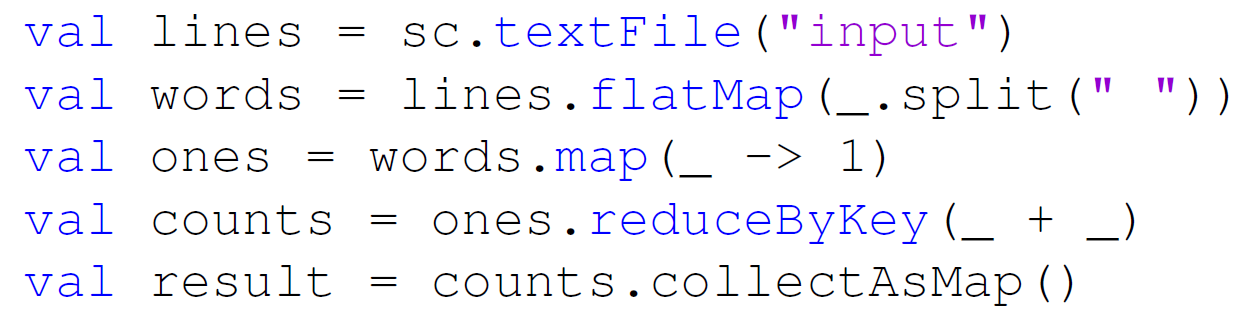
\includegraphics[width=\linewidth]{images/sparkwc.png}
			\caption{\textit{Spark word count code.}}
		\end{figure}
	\subsubsection{The DAG}
		\par
		The Directed Acyclic Graph is built from the RDD lineage. The DAG scheduler transforms the DAG into stages and turns each partition of a stage into a single task.
		\newline
		Spark tuning is the repartitioning of the initial data to fully exploit the hardware: make more tasks for more, smaller, partitions, instead of just one big partition on one task.
	\subsubsection{The execution plan}
		\par
		Spark Tasks execute serialized RDD lineage DAG plus the closures of transformations. They are run by Spark Executors.
		\newline
		The driver side task scheduler launches tasks on executors according to resources and locality constraints, it decides where to run tasks.
	\subsubsection{The Shuffle phase}
		\par
		The \textit{reducebykey} transformation induces the shuffle phase (wide dependency), intermediate key-value pairs are stored on the local file system like in Hadoop.
		\newline
		This transformation also implements map-side combiners to pre-aggregate data.